%!TEX root = ../scivis_lbaakman_bvanloon.tex
\begin{figure}[h!]
	\centering
	\begin{subfigure}{0.35\textwidth}
		\centering
		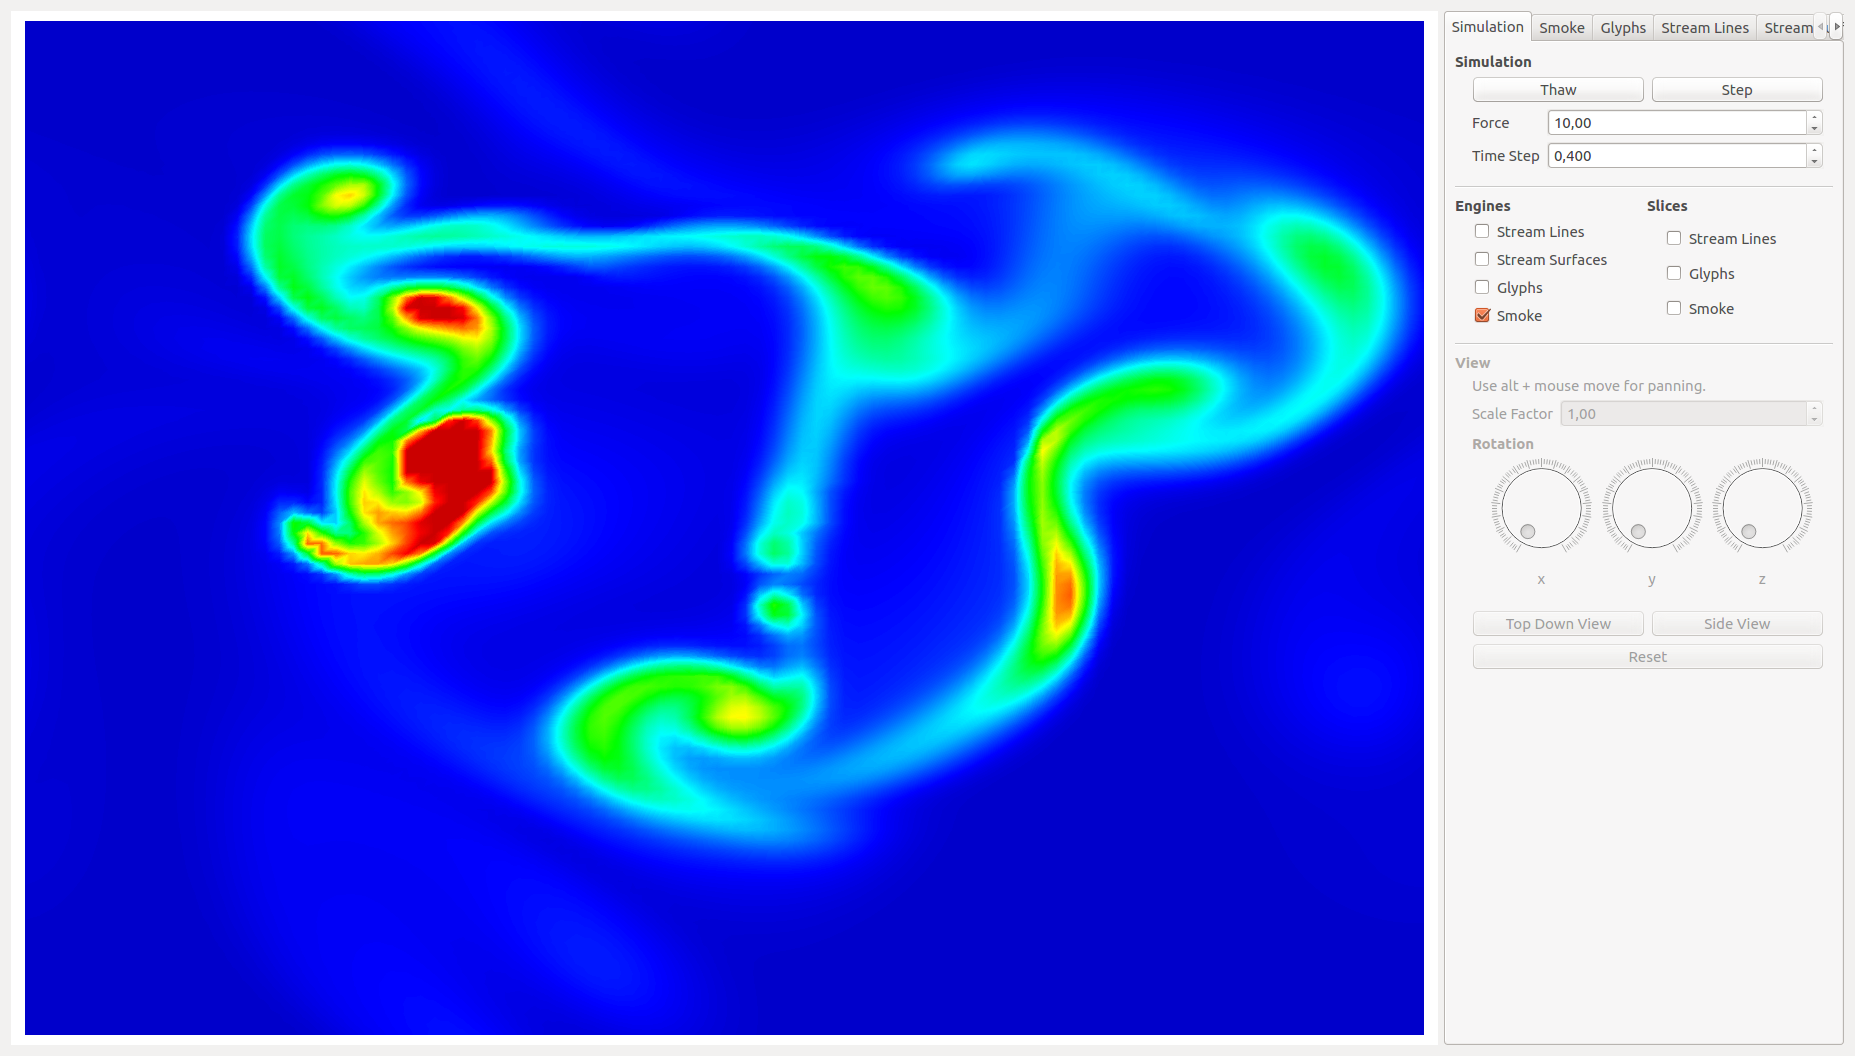
\includegraphics[width=0.9\textwidth, trim={35px 30px 430px 30px}, clip]{colormapping/img/rainbow}
		\begin{tikzpicture}
		    \node[anchor=south west,inner sep=0] (image) at (0,0) {
\includegraphics[rotate=90,width=0.03\textwidth,height=95px,keepaspectratio=false,frame]{colormapping/img/colormap_legends/rainbowcolormap}};
		\end{tikzpicture}
		\caption{Rainbow}
		\label{fig:colormapping:intro:differntColorMaps:rainbow}
	\end{subfigure}
	\hspace{30px}
	\begin{subfigure}{0.35\textwidth}
		\centering
		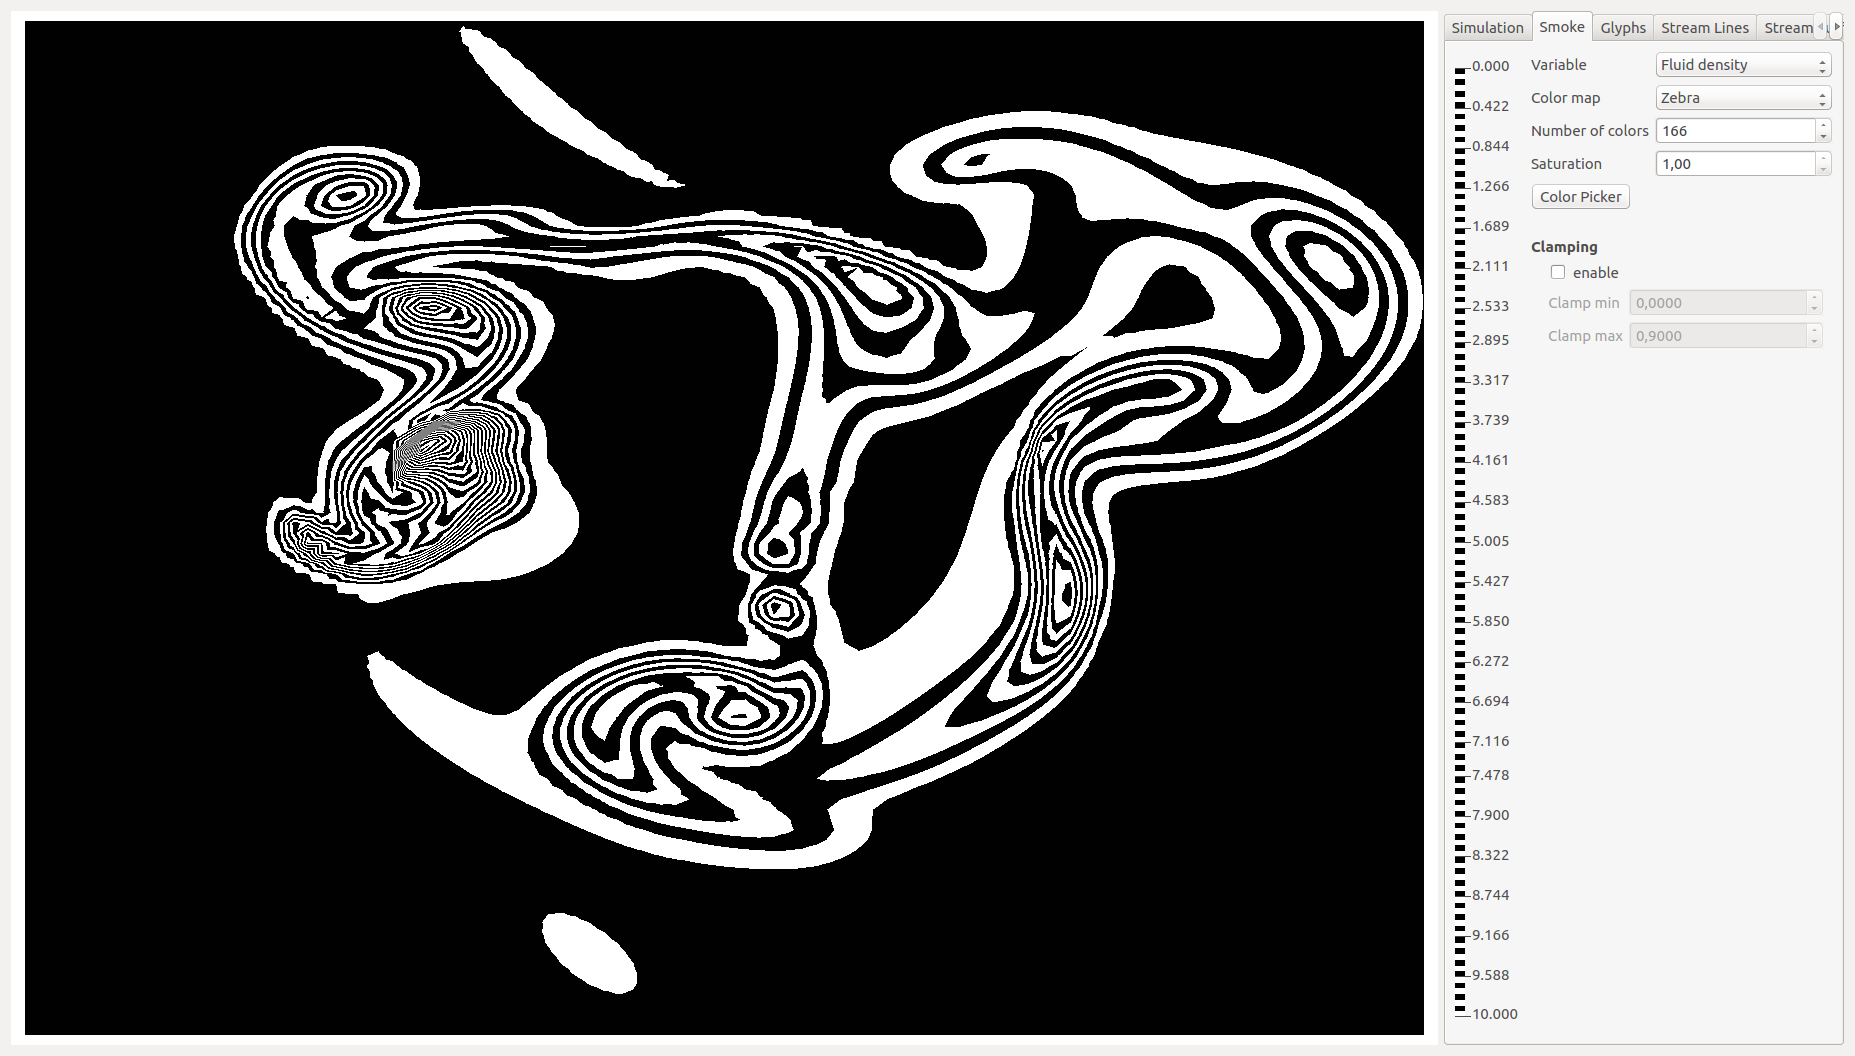
\includegraphics[width=0.9\textwidth, trim={35px 30px 430px 30px}, clip]{colormapping/img/zebra_166}
		\begin{tikzpicture}
		    \node[anchor=south west,inner sep=0] (image) at (0,0) {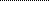
\includegraphics[rotate=90,width=0.03\textwidth,height=95px,keepaspectratio=false,frame]{colormapping/img/colormap_legends/zebracolormap}};
		\end{tikzpicture}
		\caption{Zebra}
		\label{fig:colormapping:intro:differntColorMaps:zebra}
	\end{subfigure}
	\begin{subfigure}{0.35\textwidth}
		\centering
		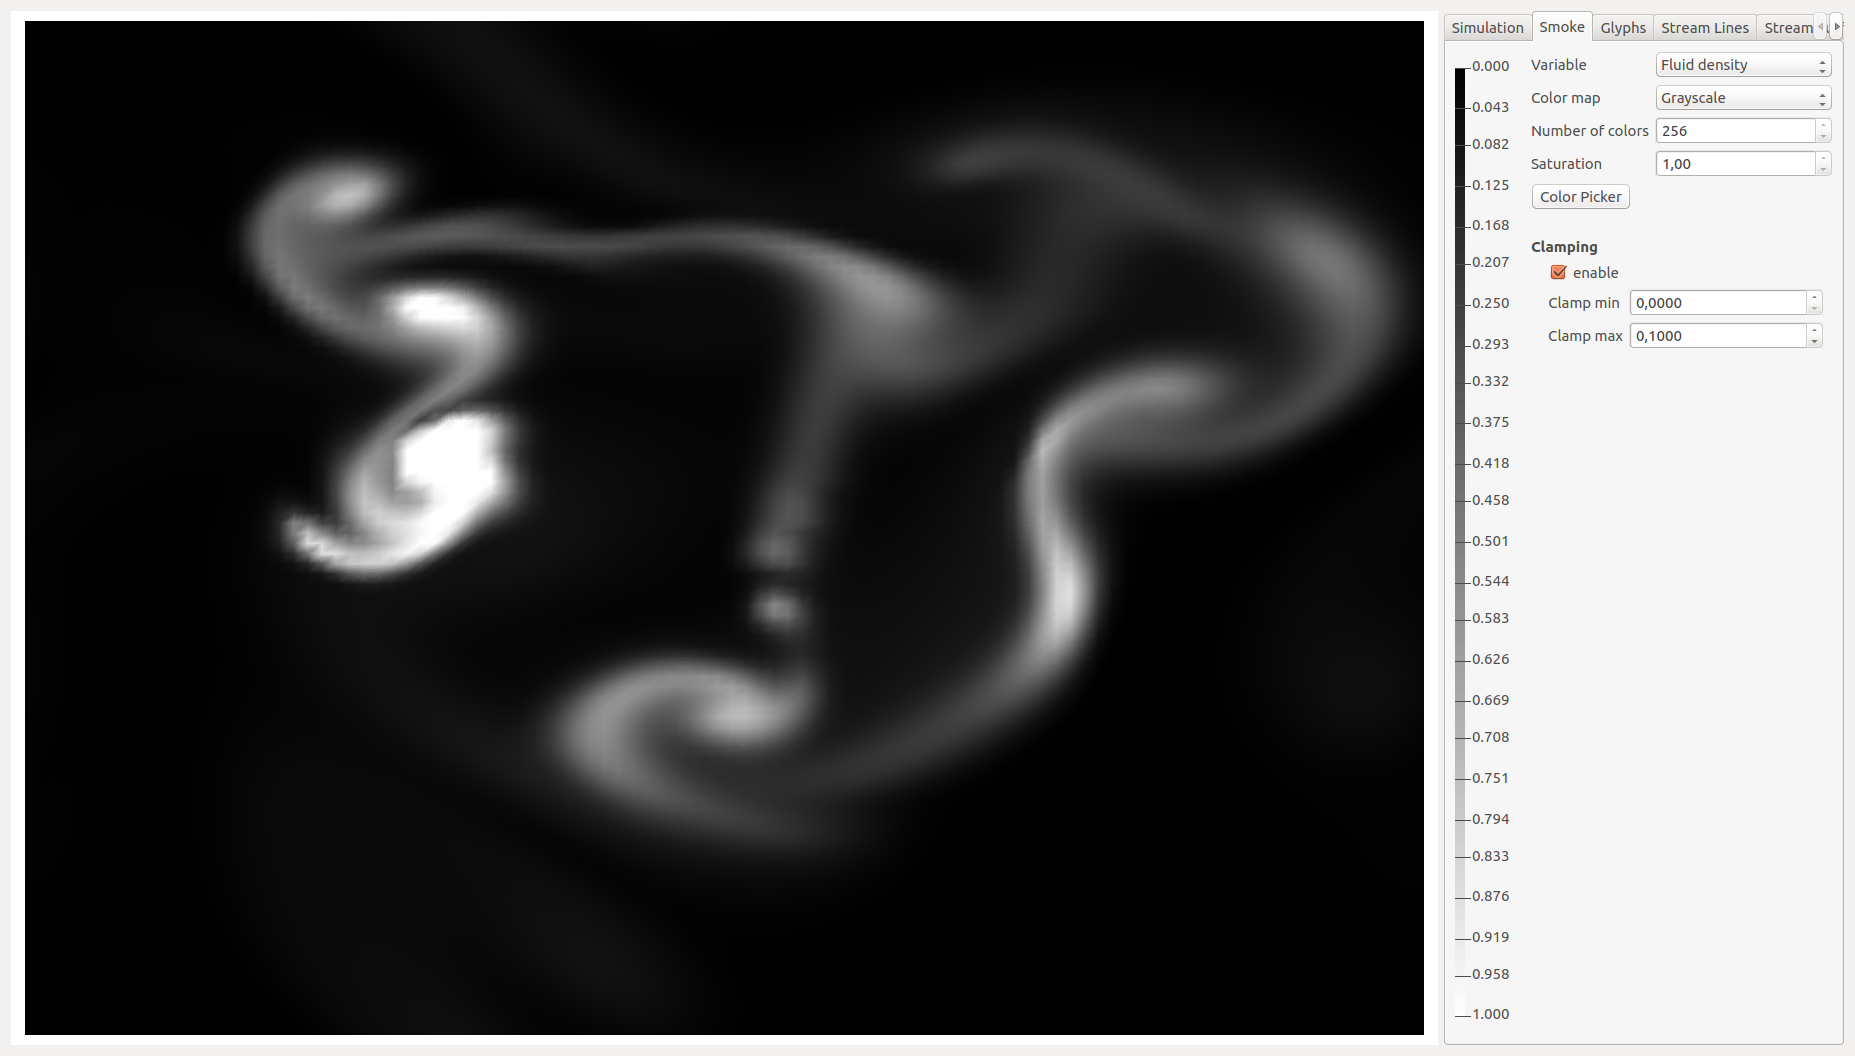
\includegraphics[width=0.9\textwidth, trim={35px 30px 430px 30px}, clip]{colormapping/img/grayscale}
		\begin{tikzpicture}
		    \node[anchor=south west,inner sep=0] (image) at (0,0) {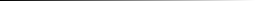
\includegraphics[rotate=90,width=0.03\textwidth,height=95px,keepaspectratio=false,frame]{colormapping/img/colormap_legends/grayscalecolormap}};
		\end{tikzpicture}
		\caption{
		Gray-scale.
		}
		\label{fig:colormapping:intro:differntColorMaps:grayscale}
	\end{subfigure}
		\hspace{30px}
	\begin{subfigure}{0.35\textwidth}
		\centering
		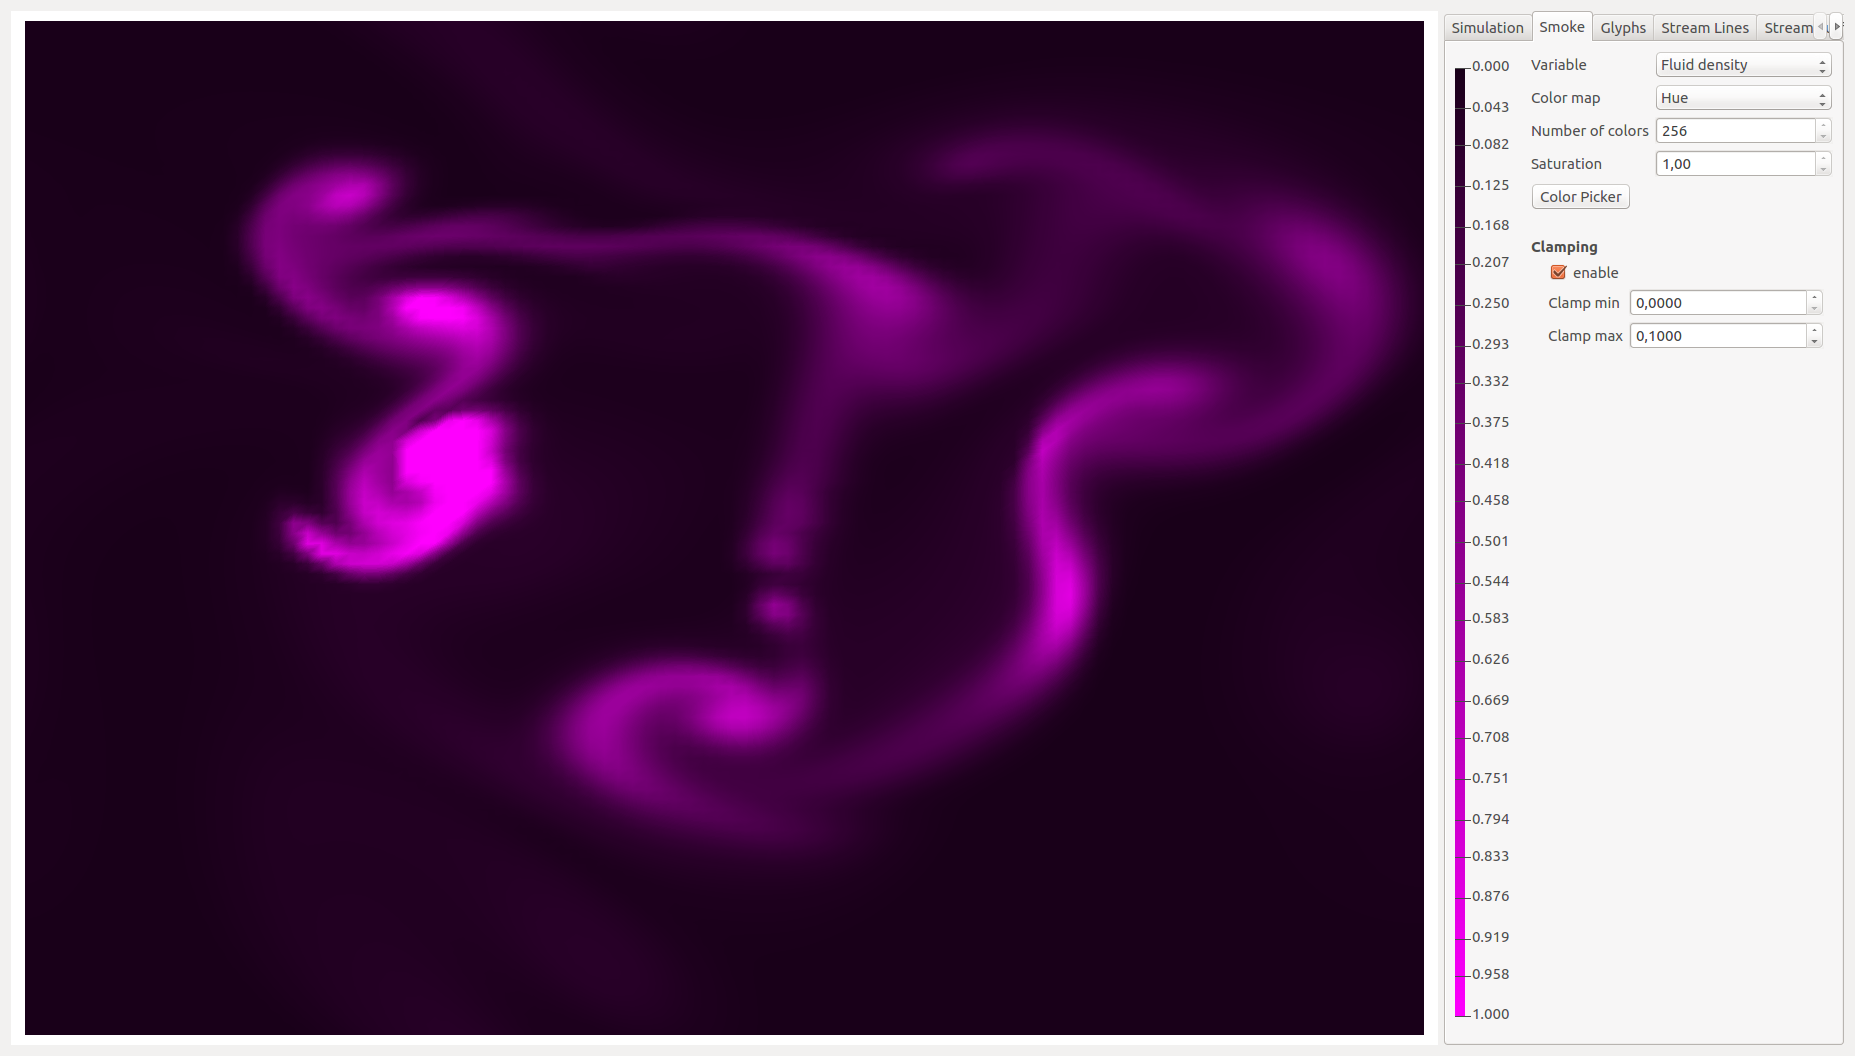
\includegraphics[width=0.9\textwidth, trim={35px 30px 430px 30px}, clip]{colormapping/img/hue}
		\begin{tikzpicture}
		    \node[anchor=south west,inner sep=0] (image) at (0,0) {
\includegraphics[rotate=90,width=0.03\textwidth,height=95px,keepaspectratio=false,frame]{colormapping/img/colormap_legends/huecolormap}};
		\end{tikzpicture}
		\caption{
		Hue (Pink)
		}
		\label{fig:colormapping:intro:differntColorMaps:hue}
	\end{subfigure}
	\begin{subfigure}{0.35\textwidth}
		\centering
		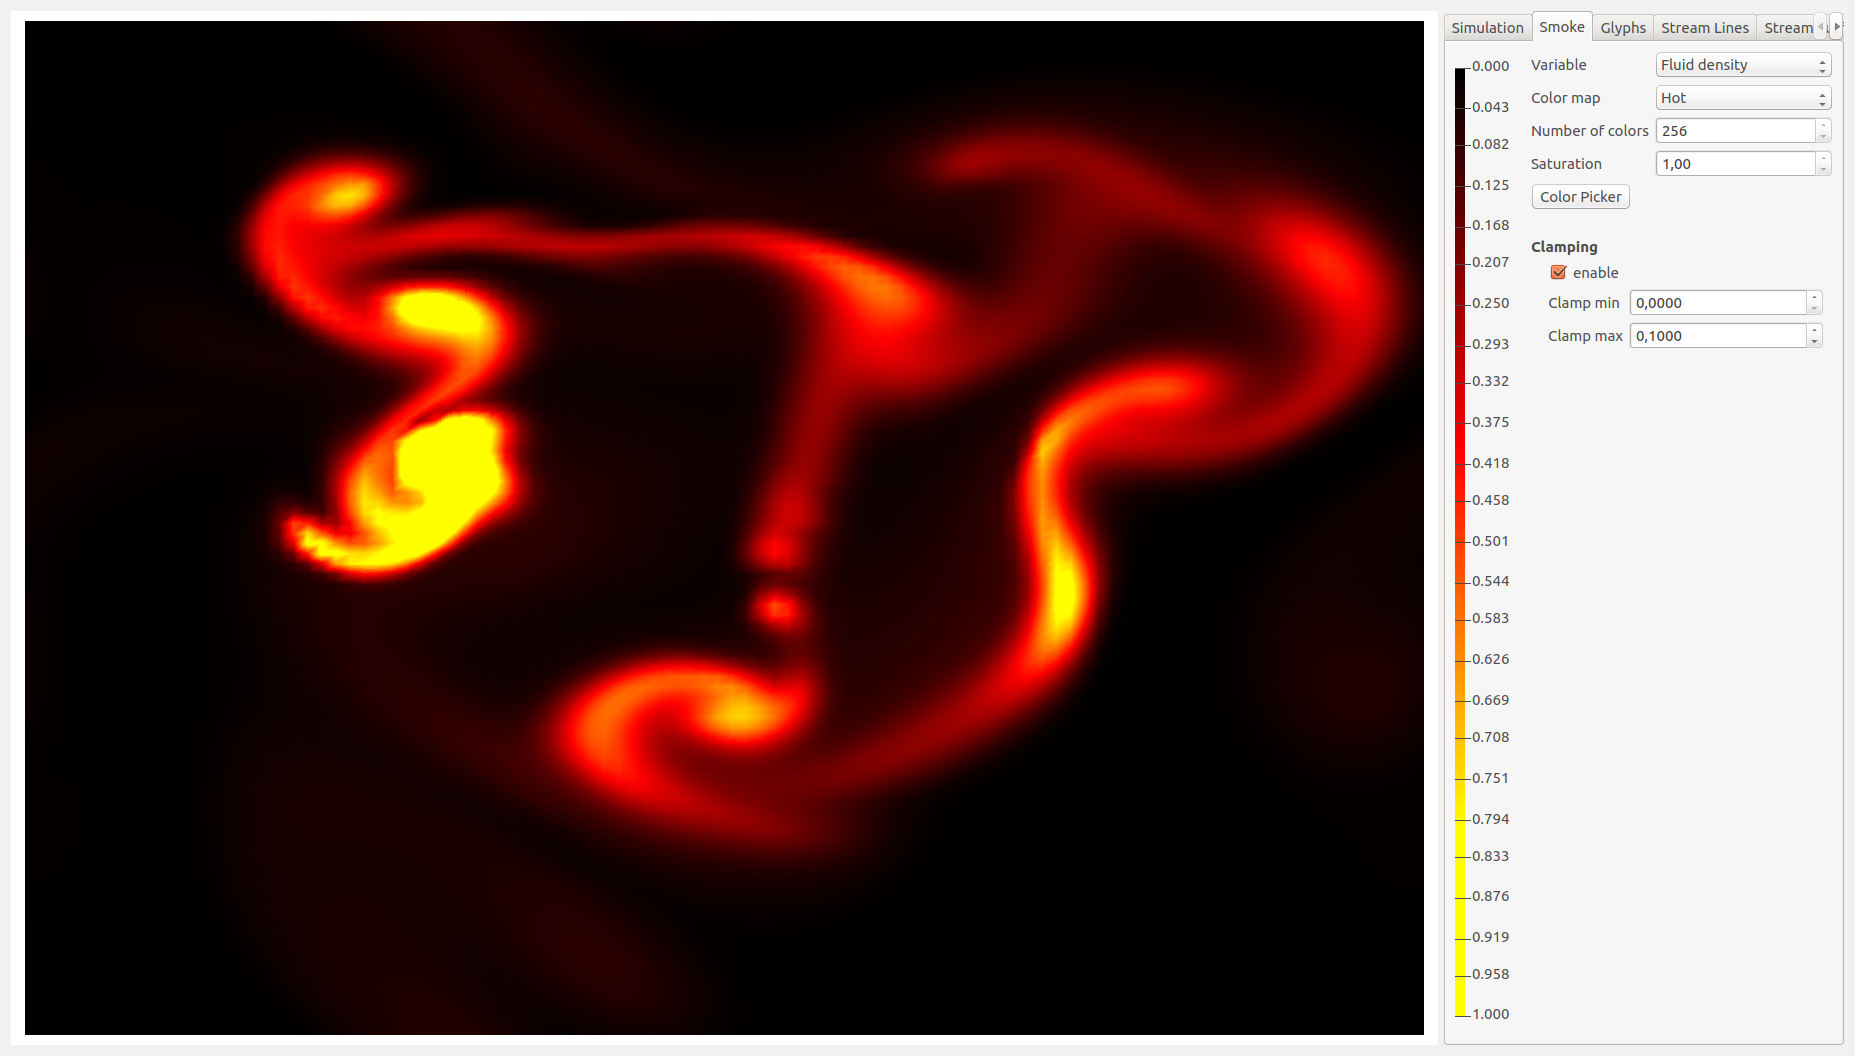
\includegraphics[width=0.9\textwidth, trim={35px 30px 430px 30px}, clip]{colormapping/img/heat}
		\begin{tikzpicture}
		    \node[anchor=south west,inner sep=0] (image) at (0,0) {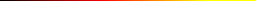
\includegraphics[rotate=90,width=0.03\textwidth,height=95px,keepaspectratio=false,frame]{colormapping/img/colormap_legends/heatcolormap}};
		\end{tikzpicture}
		\caption{
		Heat
		}
		\label{fig:colormapping:intro:differntColorMaps:heat}
	\end{subfigure}
		\hspace{30px}
	\begin{subfigure}{0.35\textwidth}
		\centering
		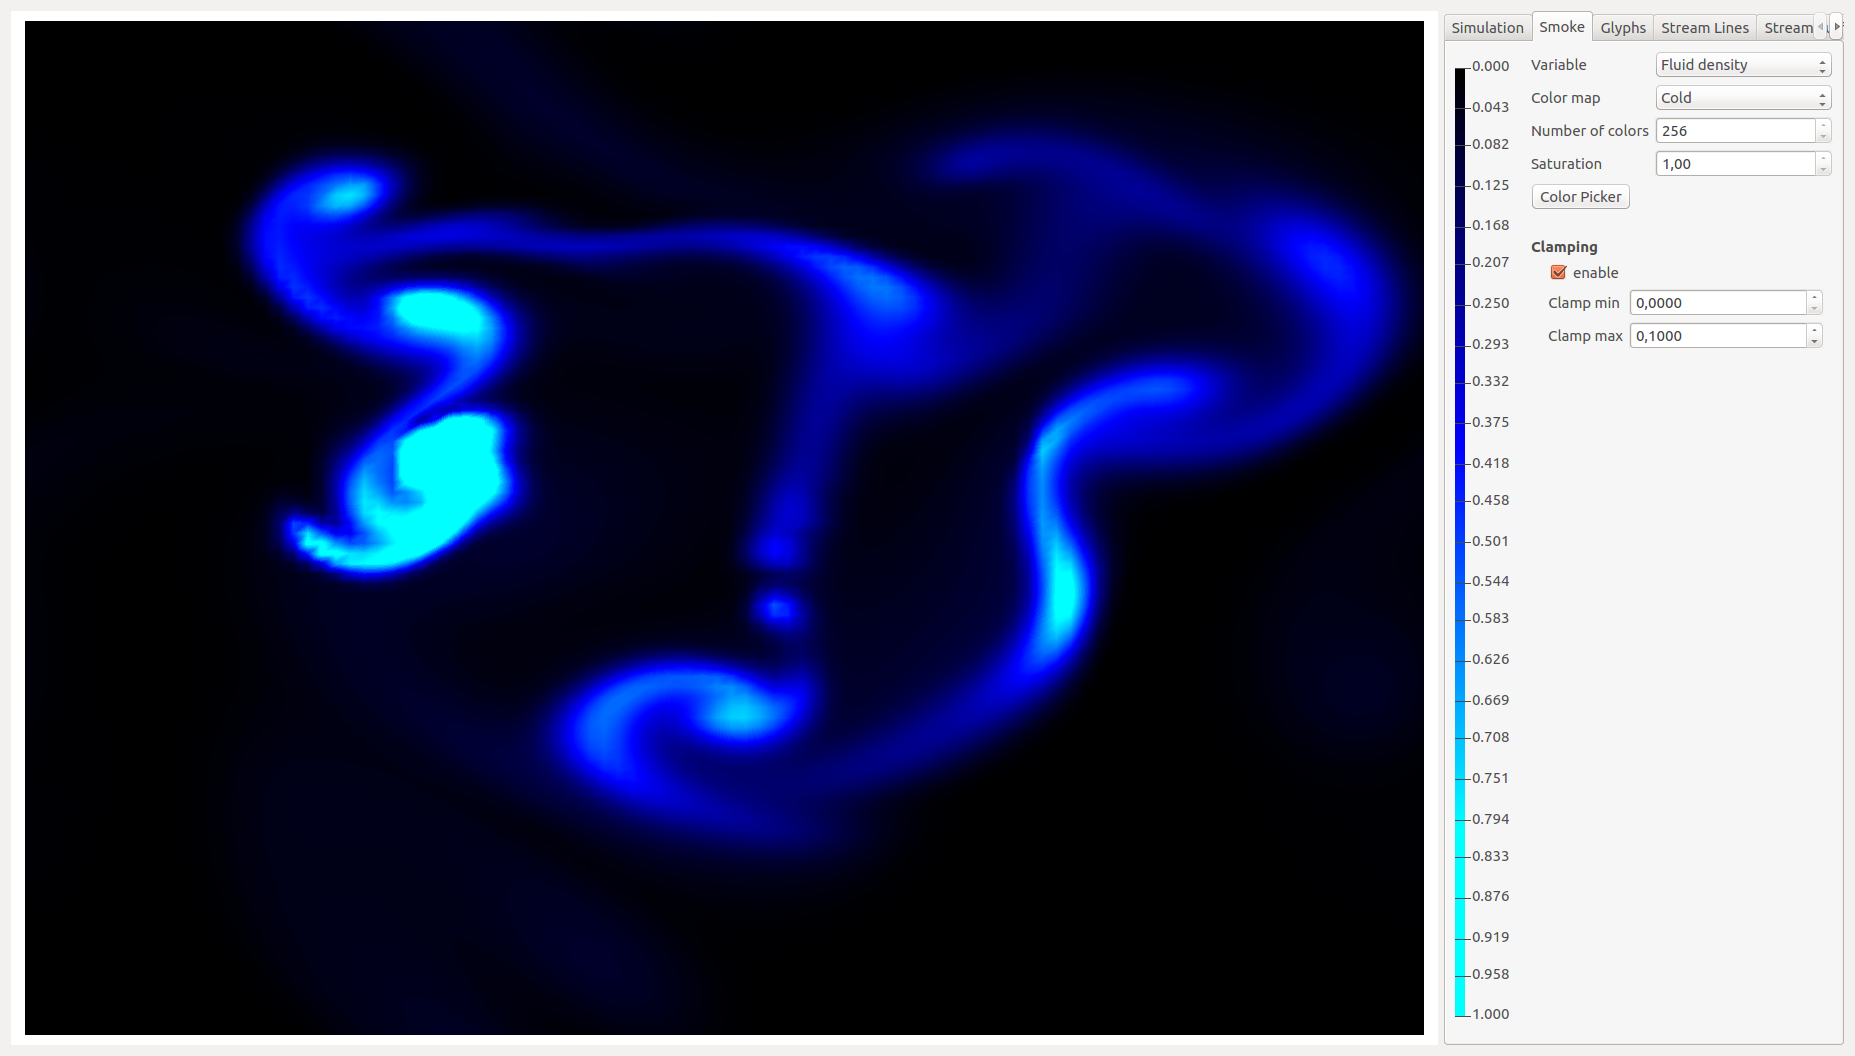
\includegraphics[width=0.9\textwidth, trim={35px 30px 430px 30px}, clip]{colormapping/img/cold}
				\begin{tikzpicture}
		    \node[anchor=south west,inner sep=0] (image) at (0,0) {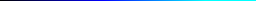
\includegraphics[rotate=90,width=0.03\textwidth,height=95px,keepaspectratio=false,frame]{colormapping/img/colormap_legends/coldcolormap}};
		\end{tikzpicture}
		\caption{
		Cold
		}
		\label{fig:colormapping:intro:differntColorMaps:cold}
	\end{subfigure}	
	\begin{subfigure}{0.35\textwidth}
		\centering
		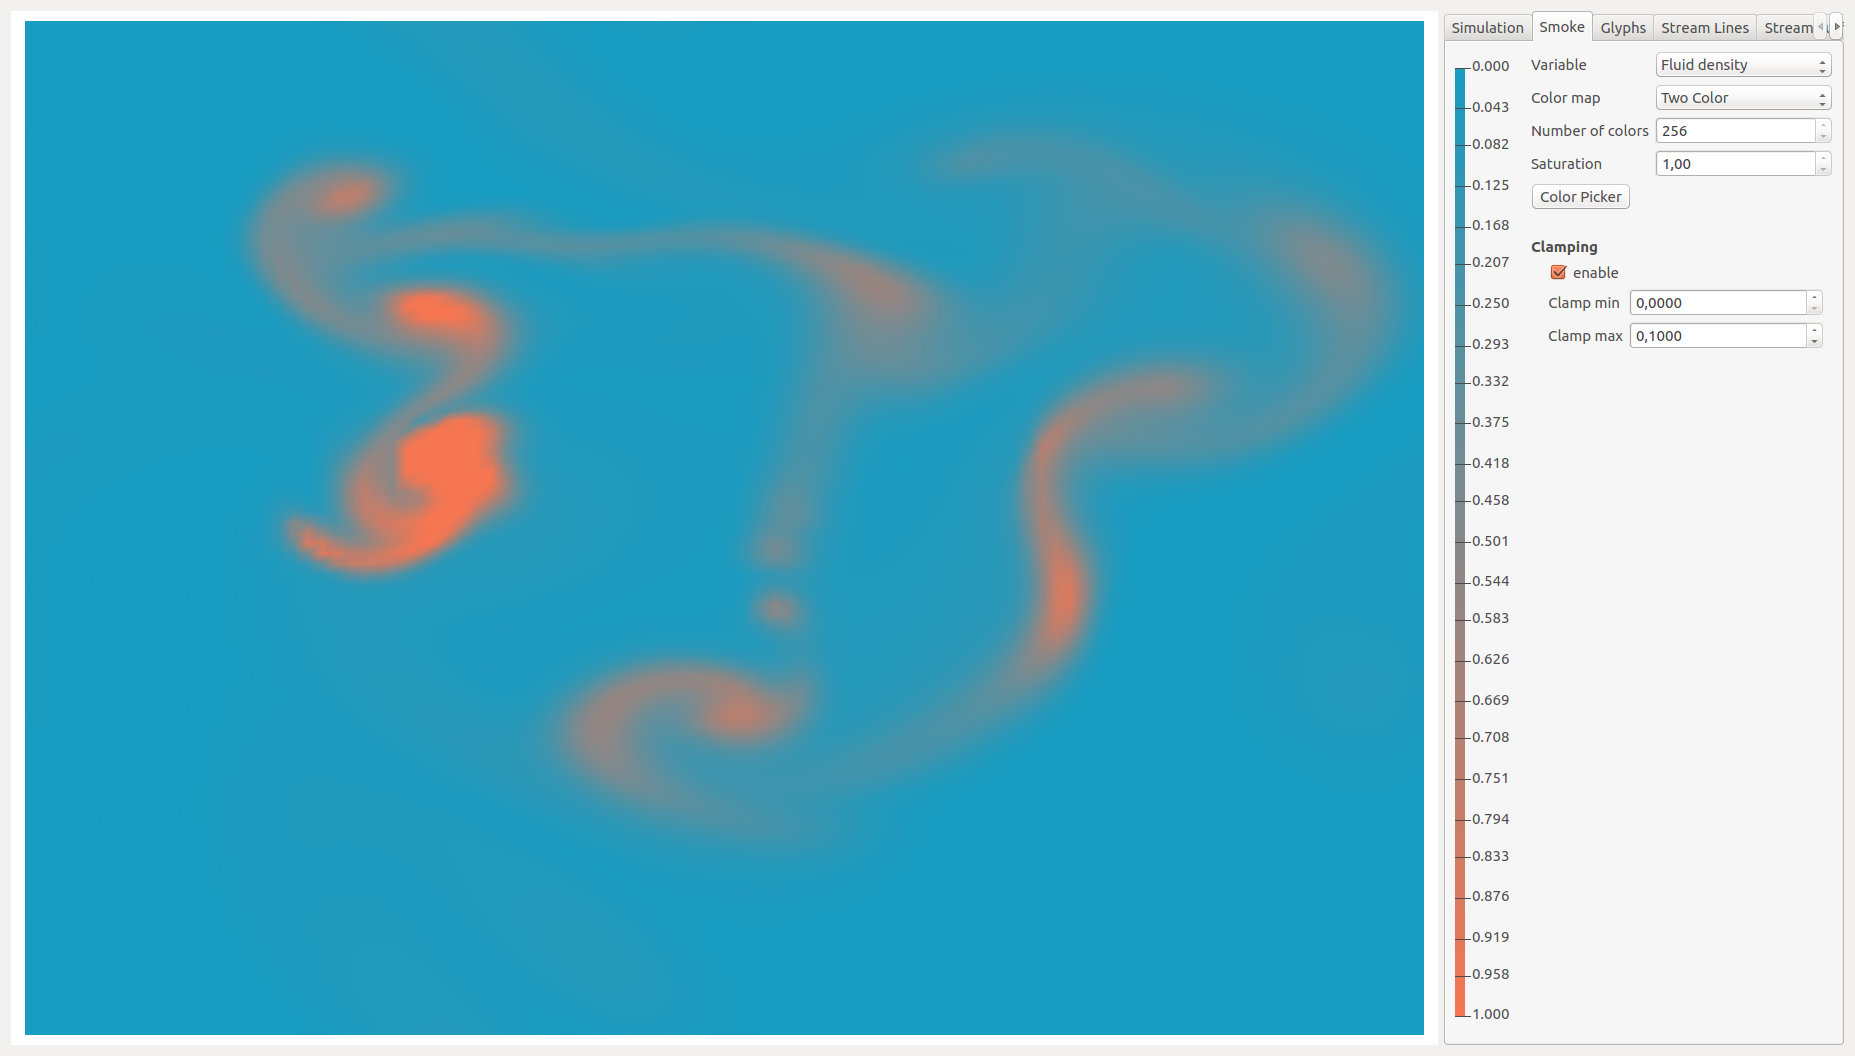
\includegraphics[width=0.9\textwidth, trim={35px 30px 430px 30px}, clip]{colormapping/img/twocolors}
		\begin{tikzpicture}
		    \node[anchor=south west,inner sep=0] (image) at (0,0) {
\includegraphics[rotate=90,width=0.03\textwidth,height=95px,keepaspectratio=false,frame]{colormapping/img/colormap_legends/twocolorscolormap}};
		\end{tikzpicture}
		\caption{
		Isoluminant Blue-Red
		}
		\label{fig:colormapping:intro:differntColorMaps:twocolor}
	\end{subfigure}	
	\hspace{30px}
	\begin{subfigure}{0.35\textwidth}
		\centering
		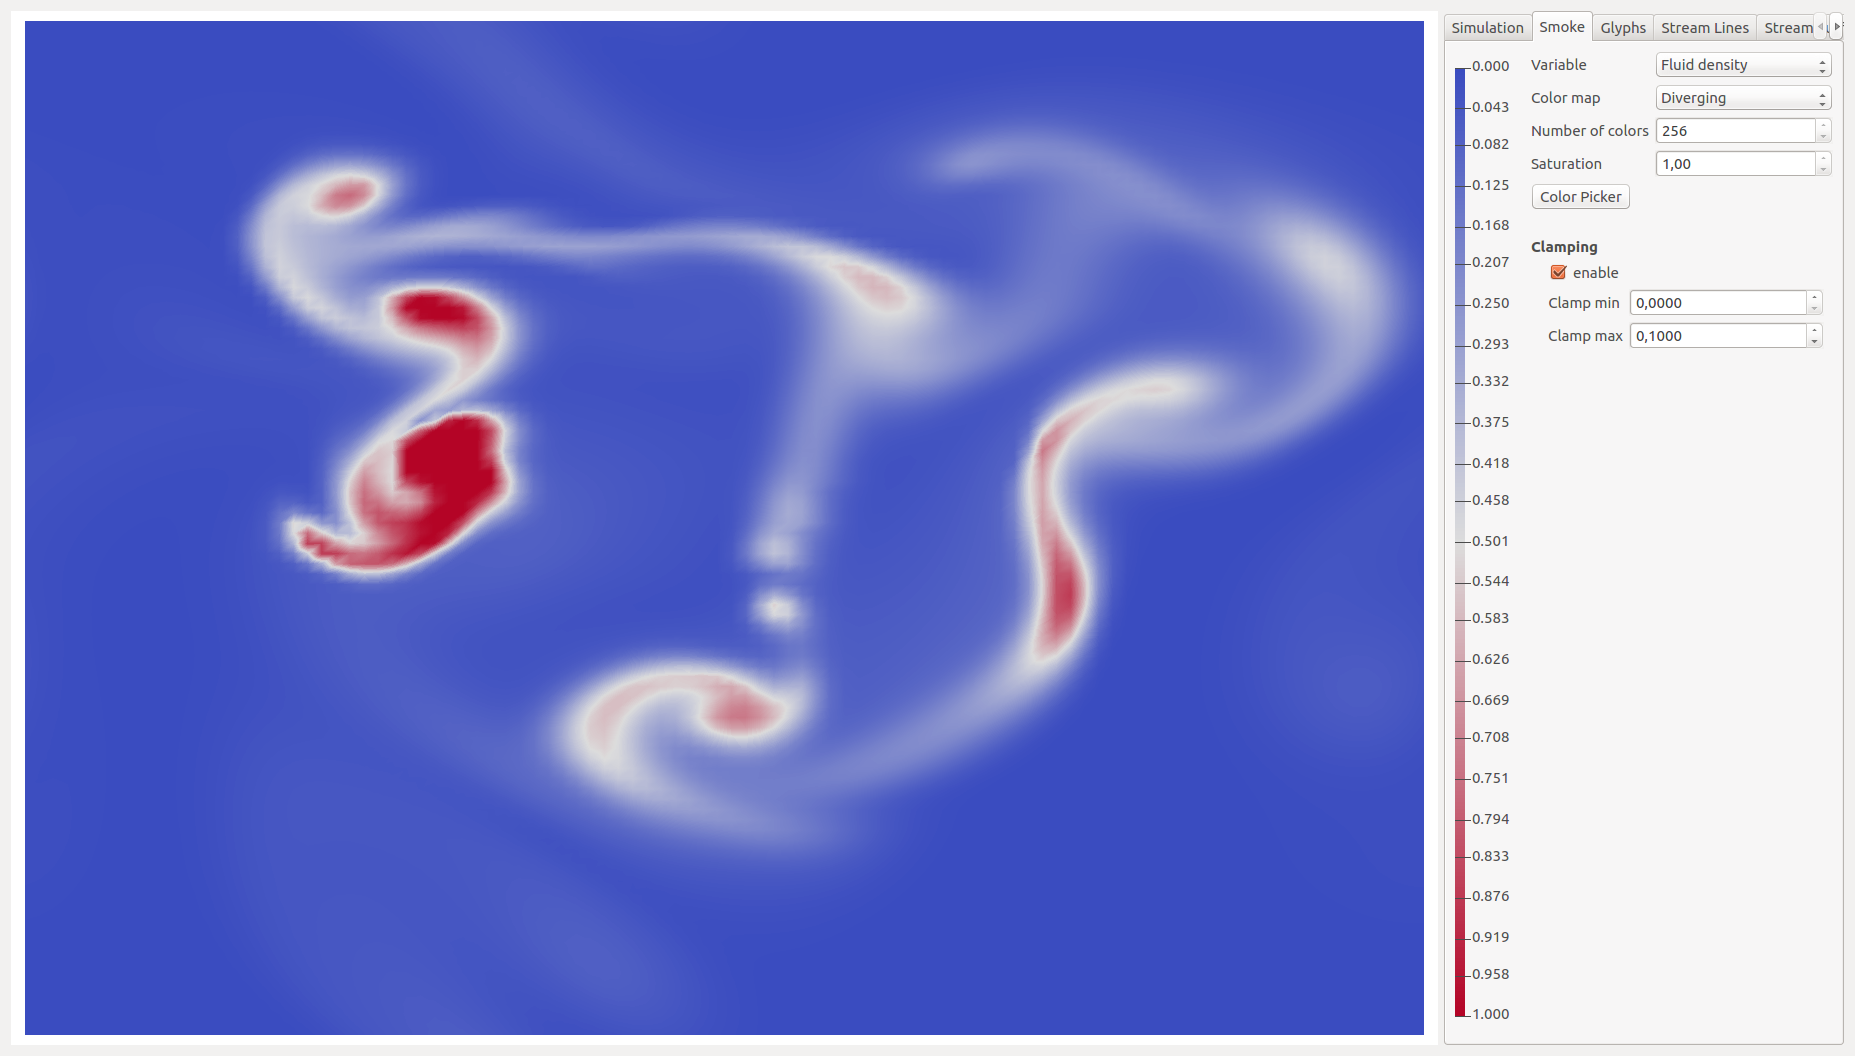
\includegraphics[width=0.9\textwidth, trim={35px 30px 430px 30px}, clip]{colormapping/img/diverging}
		\begin{tikzpicture}
		    \node[anchor=south west,inner sep=0] (image) at (0,0) {
\includegraphics[rotate=90,width=0.03\textwidth,height=95px,keepaspectratio=false,frame]{colormapping/img/colormap_legends/divergingcolormap}};
		\end{tikzpicture}
		\caption{
		Diverging
		}
		\label{fig:colormapping:intro:differntColorMaps:diverging}
	\end{subfigure}		
\caption{A visualization of the fluid density (\density) using the color maps available in the application. All color maps uses 256 colors except for the zebra color map which uses 50. All color maps are fully saturated.}
\label{fig:colormapping:colormaps}
\end{figure}


In \cref{fig:colormapping:colormaps} a visualization from simulation snapshot is shown using all the different color maps available in the application. Comparing these figures we observe firstly that in the visualization with the rainbow color map, \cref{fig:colormapping:intro:differntColorMaps:rainbow}, the maximum values are very prominent and that there is a clear distinction between the blue, green, and green areas but no clear transition between those areas. This fits with the disadvantages discussed in \cref{ssub:rainbow_colormap}. \Cref{fig:colormapping:intro:differntColorMaps:zebra} indeed illustrates the areas with high and low variation. 

Comparing the luminance based color maps, \crefrange{fig:colormapping:intro:differntColorMaps:grayscale}{fig:colormapping:intro:differntColorMaps:cold}, we observe in all cases  a nice transition and from areas with low to areas with high scalar values. Also note the added benefit of the maps containing hues compared to the gray-scale color map; especially in the areas containing low values a bit more variation is visible.


The isoluminant blue-red color map, shown in \cref{fig:colormapping:intro:differntColorMaps:twocolor}, does not offer as much details as the other color maps. This confirms that these color maps are not well suited for 2D visualizations.

In the diverging color map, illustrated in \cref{fig:colormapping:intro:differntColorMaps:diverging}, one easily recognizes the same distinct areas shown by the rainbow color map.  Compared to the rainbow color map, there are two distinct differences. First the maximum values do not draw as much attention as they do in the rainbow color map, furthermore we can see a more natural transition from low to high values making this color map more suitable for visualization of these data.